\subsection{input\_osmotr()}

Блок-схема на рисунке \ref{fig:input_osmotr}.

\begin{figure}[p]
    \center{
        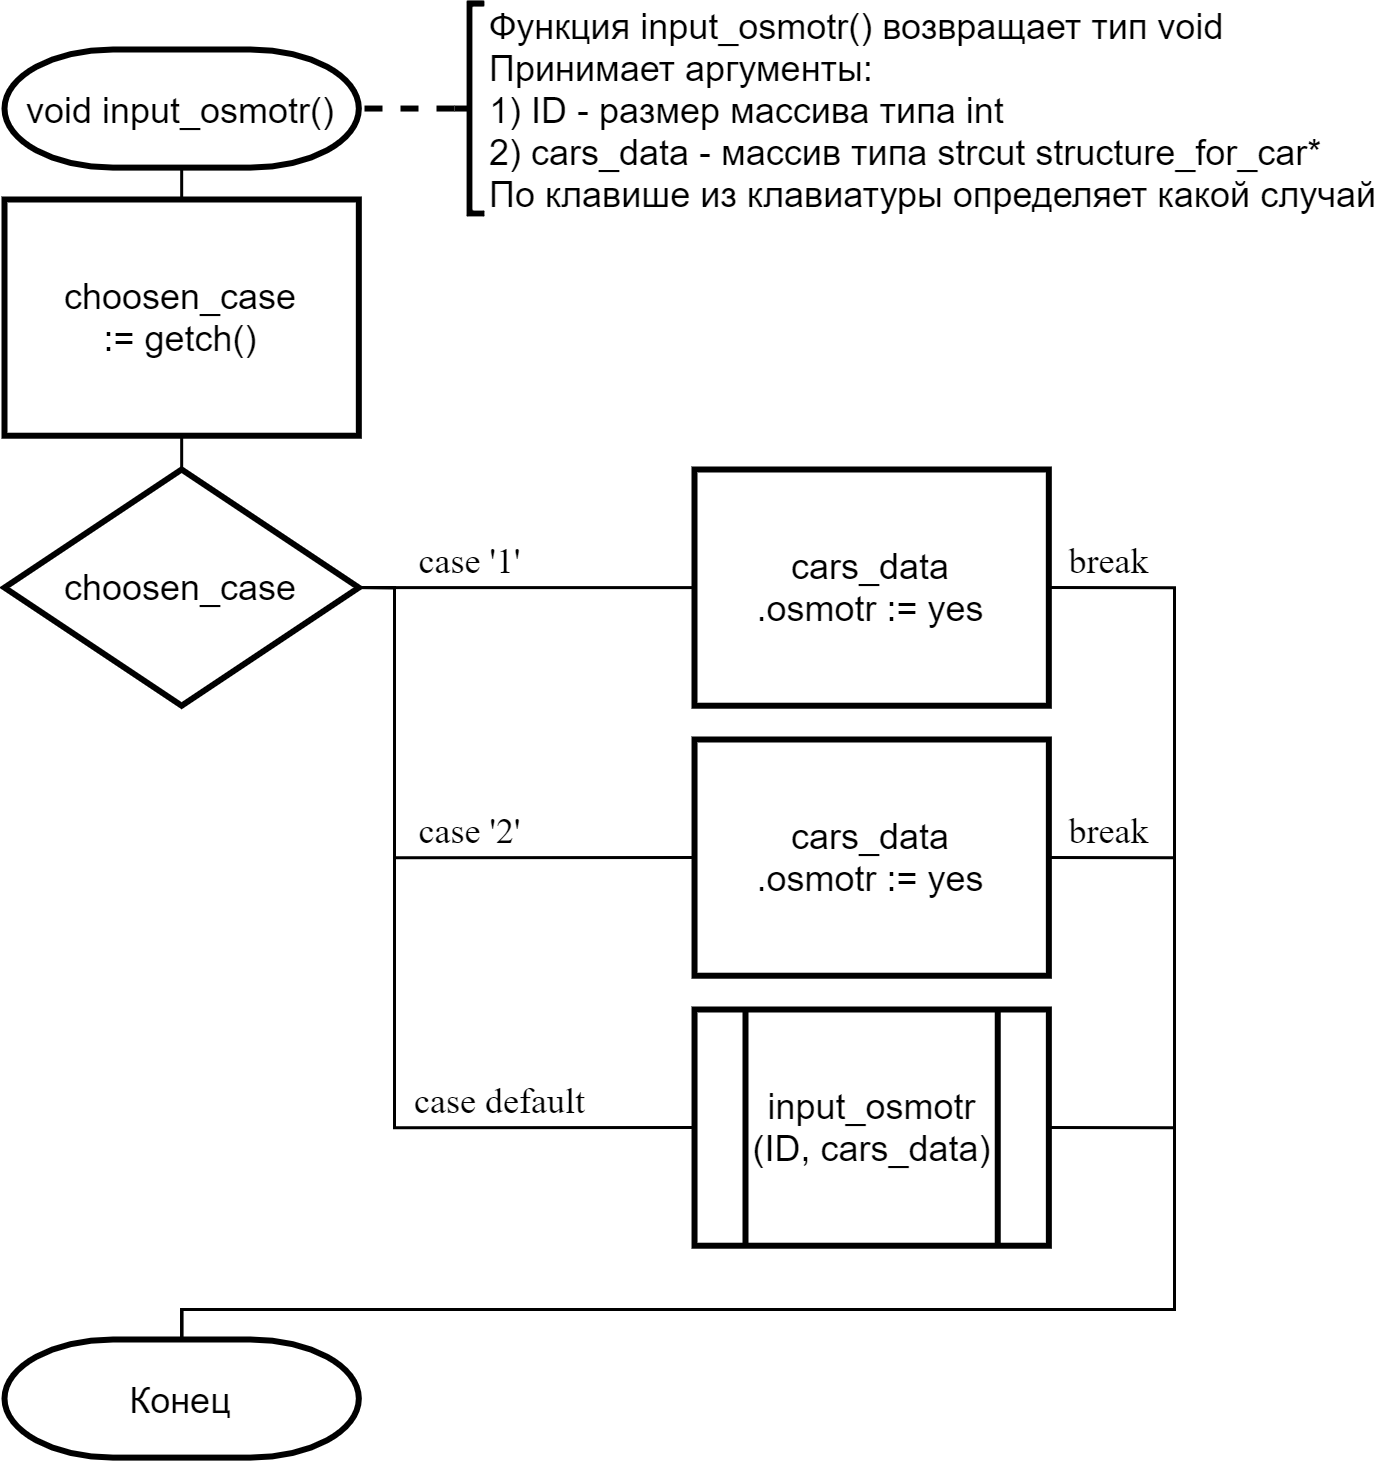
\includegraphics[width=16cm]{../13/src/lab/menu/input_data/input_osmotr/input_osmotr.png}
    }
    \caption{input\_osmotr()}
    \label{fig:input_osmotr}
\end{figure}

\lstinputlisting[
    language=C,
    name=input\_osmotr.h
]{../13/src/lab/menu/input_data/input_osmotr/input_osmotr.h}

\lstinputlisting[
    language=C,
    name=input\_osmotr.c
]{../13/src/lab/menu/input_data/input_osmotr/input_osmotr.c}

\newpage